\documentclass[12pt]{article}

%%%%%%%%%%%%%%%%%%%
% Packages/Macros %
%%%%%%%%%%%%%%%%%%%
\usepackage{amssymb,latexsym,amsmath}     % Standard packages
\usepackage{graphicx}
\usepackage{subcaption}
%\usepackage{subfig}
%\usepackage[caption=false]{subfig}
\usepackage{cite} % Allows for ranges in citation
\usepackage{mciteplus}
\usepackage[toc,page]{appendix}
\usepackage{titlesec}
\usepackage{xcolor}
\usepackage{hyperref}    % Hyperlinks in references
%\usepackage[all]{hypcap} % Internal hyperlinks to floats.
\definecolor{darkblue}{rgb}{0,0,0}
\definecolor{darkgreen}{rgb}{0,0.5,0}
\definecolor{darkviolet}{rgb}{0.55,0.,0.55}
\hypersetup{colorlinks=true, linkcolor=darkblue, citecolor=darkviolet, urlcolor=darkgray}
\usepackage{array}
\usepackage{booktabs}
%%%%%%%%%%%
% Margins %
%%%%%%%%%%%
%\addtolength{\textwidth}{2.3in}
%\addtolength{\textheight}{2.3in}
%\addtolength{\evensidemargin}{-0.2in}
%\addtolength{\oddsidemargin}{-0.2in}
%\addtolength{\topmargin}{-1.2in}
%\usepackage[usenames,dvipsnames,svgnames,table]{xcolor}

%%%%%%%%%%%%%%%%%%%%%%%%%%%%%%
% Theorem/Proof Environments %
%%%%%%%%%%%%%%%%%%%%%%%%%%%%%%
\newtheorem{theorem}{Theorem}
\newenvironment{proof}{\noindent{\bf Proof:}}{$\hfill \Box$ \vspace{10pt}}  


%%%%%%%%%%%%
% Document %
%%%%%%%%%%%%
\begin{document}

\title{\textit{GateParamterisedPinholeCollimator} class for simulation of preclinical SPECT}
%\author{}
\maketitle
\tableofcontents
\newpage
%\begin{abstract}
%\end{abstract}



\pagebreak


%%%%%%%%%%%%%%%%%%%%%%%%%%%%%%%%%%%%%%%%%%%%%%%%%%%
\section{Aim}
This class was developed for simulations of a nanoSPECT/CT~(Fig.~\ref{fig:scanner}) by Mediso with a pinhole collimator~(Fig.~\ref{fig:colli}).
 
\begin{figure}[htp]
\centering
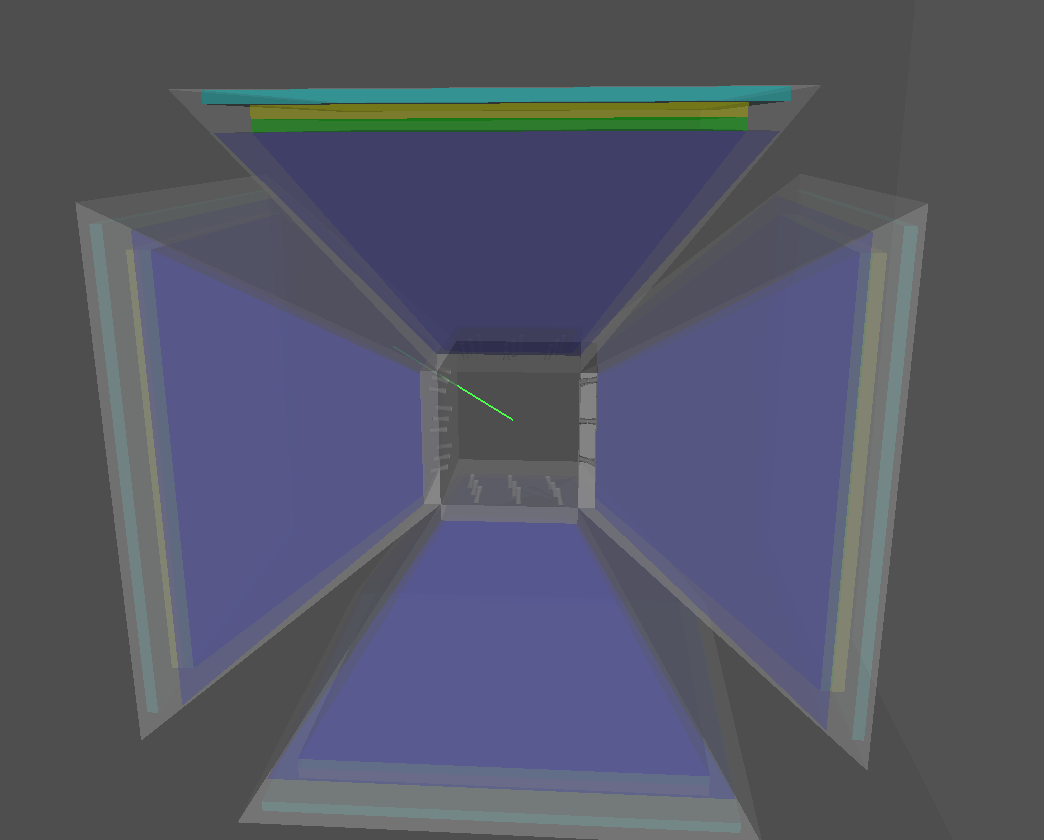
\includegraphics[scale=0.3]{figs/scanner.png}
\caption{Illustration for simulated nanoSPECT}
\label{fig:scanner}
\end{figure}

\begin{figure}[htp]
\centering
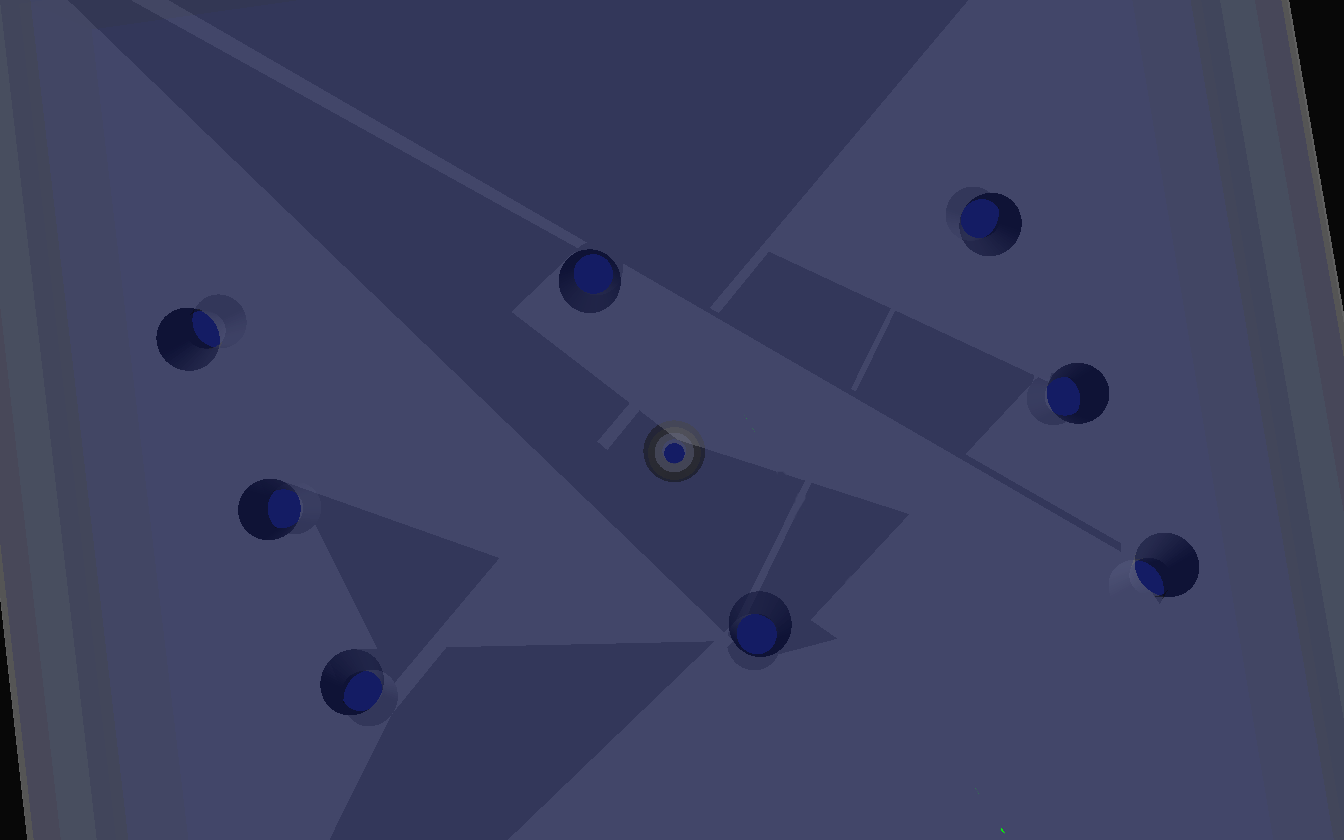
\includegraphics[scale=0.3]{figs/colli.png}
\caption{Illustration for pinhole collimator}
\label{fig:colli}
\end{figure}


\section{Options and input data}
The geometry of pinhole is defined from a G4-pyramid with a subtracted cones in order to have pinholes.

The pyramid is defied with mac options:  
\begin{verbatim}
/gate/colli/geometry/setDimensionX1 80 mm
/gate/colli/geometry/setDimensionY1 84 mm
/gate/colli/geometry/setDimensionX2 80 mm
/gate/colli/geometry/setDimensionY2 84 mm
/gate/colli/geometry/setHeight 10 mm
\end{verbatim}

The collimator rotation radius, i.e. distance from the center of field of view to the pinholes center (see Fig.~\ref{fig:rot_radius} and Fig,~\ref{fig:pinhole}) is defined as:
\begin{verbatim}
/gate/colli/geometry/setRotRadius 45 mm
\end{verbatim}

\begin{figure}[htp]
\centering
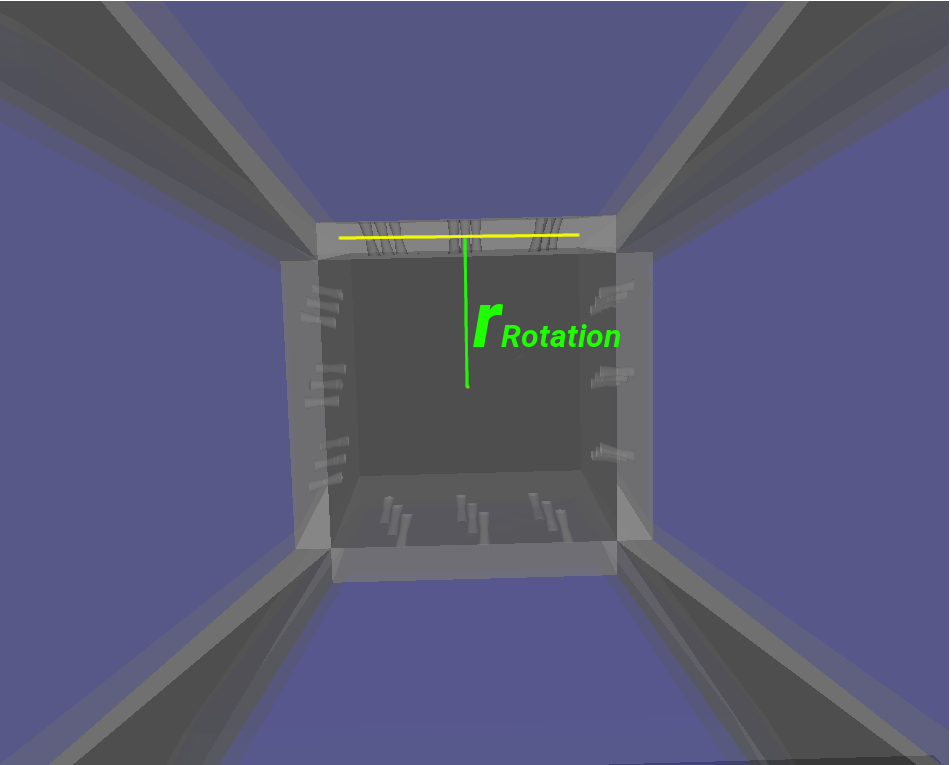
\includegraphics[scale=0.3]{figs/rot_radius.png}
\caption{Definition of the rotation radius}
\label{fig:rot_radius}
\end{figure}


The the pinhole geometry is defined with an option file:
\begin{verbatim}
/gate/colli/geometry/input mac/APT2.pin
\end{verbatim}

The stricture of the option file, APT2.pin, is the following (an example could be found in Table~\ref{tab:ResTUBES}):
\begin{verbatim}
Number of pinholes
y	z	diameter cone_angle	focal_point_y focal_point_z
\end{verbatim}

 \begin{table}[ht]
 \begin{center}
     \begin{tabular}{cccccc}
      \#~~ y & z & dia & cone & focal & point \\
	  {[APT2]} &  & &  &  &  \\
	   9 &  & &  &  &  \\
	   -28.5 & 12.0 & 2.5 & 6.3 & -18.5 & 0 \\
		-3.5 & 12.0 & 2.5 & 6.3 & -3.5 & 0 \\
		21.5 & 12.0 & 2.5 & 6.3 & 11.5 & 0 \\
		-25.0 & 0 & 2.5 & 6.3 & -15 & 0 \\
		0     & 0 & 2.5 & 6.3 & 0 & 0 \\
		25.0  & 0 & 2.5 & 6.3 & 15 & 0 \\
		-21.5 & -12.0 & 2.5 & 6.3 & -11.5 & 0 \\
		3.5   & -12.0 & 2.5 & 6.3 & 3.5  & 0 \\
		28.5 & -12.0 & 2.5 & 6.3 & 18.5 & 0 \\
     
     \end{tabular}
     \caption{Example of APT2.pin option file}
     \label{tab:ResTUBES}
  \end{center}
  \end{table}
In Table~\ref{tab:ResTUBES} one can find a description of APT2 collimator with 9 holes. The diameter of pinholes (at the center) is 2.5~mm, the opening cone angle ($\alpha$ later) is 6.3~degree. The y and z coordinates are the centers of the pinholes. The focal coordinates are illustrated in Fig.~\ref{fig:pinhole}.
\begin{figure}[htp]
\centering
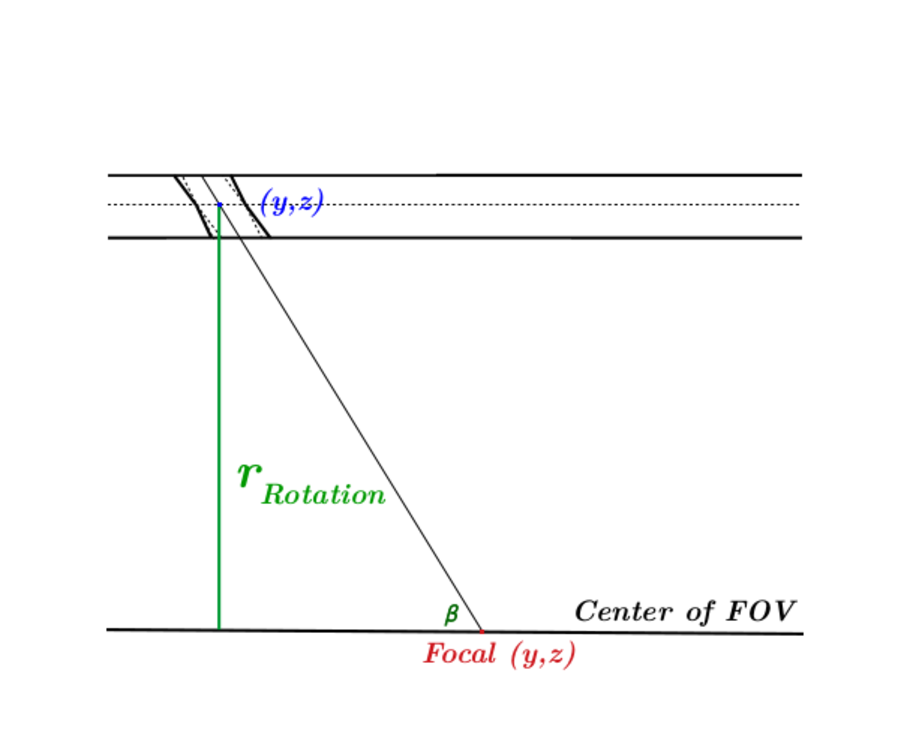
\includegraphics[scale=0.7]{figs/pinhole.pdf}
\caption{Illustration of parameters defined in APT2.pin option file}
\label{fig:pinhole}
\end{figure}


\clearpage
\section{Pinhole geometry calculations}
The result of the following calculations are implemented in GateParametrisedPinhole class.

\subsection{Cone parameters}
The names of the variables in the class are the same as in Figure~\ref{fig:fig_def_size}.
The known parameters are: \textbf{\textit{d ( = dia)}} - diameter of the pinhole, $\mathbf{\alpha}$ = cone opening angle or apex/2, $\mathbf{\beta = 90^{\circ} - \alpha}$, h = half of a thickness of collimator plate.

\begin{figure}[htp]
\centering
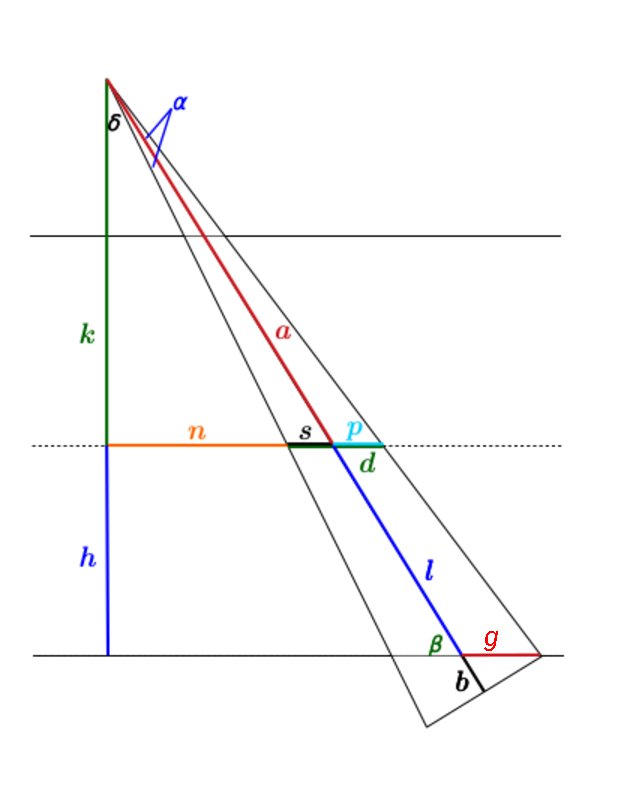
\includegraphics[scale=1]{figs/fig_def_size.pdf}
\caption{Illustration for pinhole size parameter definitions}
\label{fig:fig_def_size}
\end{figure}
\begin{enumerate}
\item Calculation of $l$
	$$\sin{\beta}=\frac{h}{l}$$
	$$l=\frac{h}{\sin{\beta}}$$
\item Calculation of $k$ and $n$
	$$\delta=90^{o}-(\alpha+\beta)$$

	\[
	\left \{
	\begin{array}{c @{=} c}
    \tan\delta = \frac{1}{\tan(\alpha+\beta)}& \frac{n}{k} \\
   	\tan(\delta+2\alpha) = \frac{1}{\tan(\beta-\alpha)} & \frac{n+d}{k} \\
	\end{array}
	\right.
	\]
	
	\[
	\left \{
	\begin{array}{c @{=} c}
    \tan(\alpha+\beta)& \frac{k}{n} \\
   	\tan(\beta-\alpha) & \frac{k}{n+d} \\
	\end{array}
	\right.
	\]
	
%	$$n=\frac{d\cdot\tan(\beta-\alpha)}{\tan(\alpha+\beta) - 	\tan(\beta-\alpha)}	$$	
	
\begin{equation} 	
	\boxed{k=\frac{d\cdot\tan(\beta-\alpha)\cdot\tan(\alpha+\beta)}{\tan(\alpha+\beta) - 	\tan(\beta-\alpha)}}
\end{equation}	
\begin{equation} 	
	\boxed{n=\frac{k}{\tan(\beta-\alpha)} - d}
	\end{equation}	
		
%and
%\begin{equation} 		
%  \boxed{k_{central}=\frac{d}{2\cdot\tan\alpha}}
%  	\end{equation}	
%  \begin{equation} 		
%	\boxed{n_{central}=0	}
%	\end{equation}	
%	
\item Calculation of $a$ from $k$ and $n$
	$$a=\frac{k}{\cos(\delta+\alpha)}=\frac{k}{\sin\beta}$$
	  \begin{equation} 	
	\boxed{a=\frac{k}{\sin\beta}}
	\end{equation}
\item 				
	$$l=\frac{h}{\cos(\delta+\alpha)}=\frac{h}{\sin\beta}$$
	  \begin{equation} 	
	\boxed{l=\frac{h}{\sin\beta}}
	\end{equation}
\item Calculation of $b$ 
	$$\tan(\delta+\alpha)=\frac{1}{\tan{\beta}} =\frac{n+s}{k}$$
	  \begin{equation} 	
	\boxed{s=\frac{k}{\tan{\beta}}-n}
	\end{equation}
	$$p=d-s$$
	$$\frac{p}{g}=\frac{a}{a+l}$$
	$$g=\frac{(d-s)\cdot(a+l)}{a}$$ 
	$$\cos\beta=\frac{b}{g}$$
	  \begin{equation} 	
	\boxed{b=\frac{(d-s)\cdot(a+l)\cdot\cos\beta}{a}}
	\end{equation}
\item Calculation of $apex$ for a chosen direction ($x$ or $y$)
\begin{equation} 
	\boxed{apex=a+l+b}			
\end{equation}	
\item In more general case: 
\begin{equation} 
	\boxed{apex=\sqrt{apex_{x}^{2}+apex_{y}^{2}}}			
\end{equation}


	
\end{enumerate}

 
 
 
\subsection{Cone positions}
 
\begin{figure}[htp]
\centering
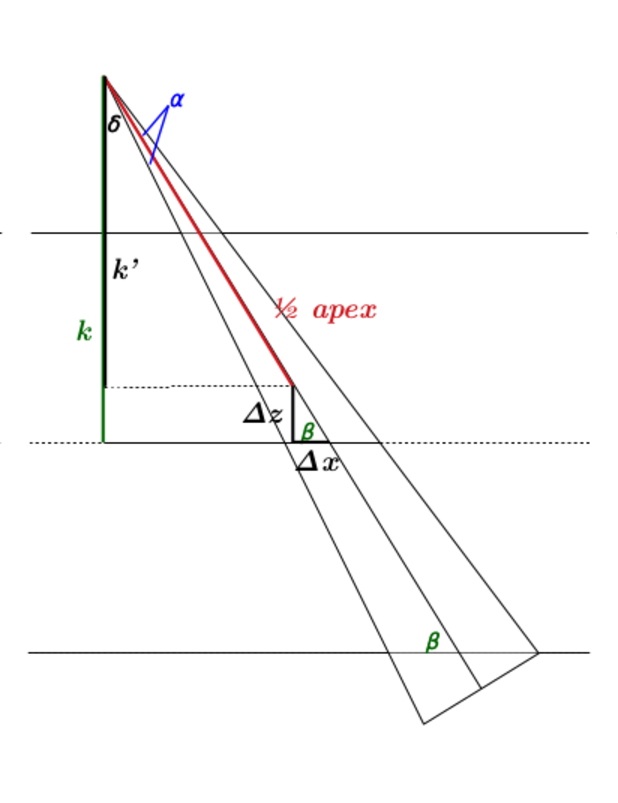
\includegraphics[scale=1]{figs/fig_def_positions.pdf}
\caption{Illustration for pinhole positions definitions}
\label{fig:fig_def_positions}
\end{figure}
According to illustration Fig.~\ref{fig:fig_def_positions}: 
\begin{enumerate}
\item Calculation of $\Delta z$
	\begin{equation} 
	\Delta z = k-k'		
	\end{equation}
	\begin{equation} 
	\cos{(\delta+\alpha)} = \sin{\beta} = \frac{k'}{apex/2}	
	\end{equation}
	\begin{equation} 
	k' = (apex/2)\cdot\sin{\beta} 
	\end{equation}
	\begin{equation} 
	\boxed{\Delta z = k - (apex/2)\cdot \sin{\beta} }		
	\end{equation}
\item Calculation of $\Delta x$ or $\Delta y$ in 3D with $\phi$ as an azimuthal angle:
	\begin{equation} 
	\boxed{\Delta x = \sin{\phi}\frac{\Delta z}{\tan{\beta}}}
	\end{equation}
	\begin{equation}	
	\boxed{\Delta y =\cos{\phi} \frac{\Delta z}{\tan{\beta}}}		
	\end{equation}
\end{enumerate}
\clearpage

\section{How to obtain .pin file}
One of tricky steps is to obtain the .pin file, i.e. pinhole parameters: positions, diameters, cone opening angles and focal points positions. 

\subsection{Input from HiSPECT reconstruction software}
Here one can find a description of how it was done for one of projects where the simulation of nanoSPECT/CT by Mediso. It is four head camera with several pinhole exchangeable collimators. In our case we were interested in APT1, a collimator for mouse imagning, and APT2, a collimator for rat imagning. 

The best way that we found was to search information in integrated reconstruction software of the scanner. In our case it was \textbf{HiSPECT}.
The pinhole information was stored in (Figure~\ref{fig:HiSPECT4det})
\begin{verbatim}
Scivis/HiSPECT/SQL/Install/NanoSPECT_Aperture_4det.sql
\end{verbatim}
In Figure~\ref{fig:HiSPECT4det}, the lines corresponding to APT1 and APT2 apertures are highlighted.

The explanations of corresponding table structures were located in 
\begin{verbatim}
Scivis/HiSPECT/SQL/Install/HiSPECT.sql
\end{verbatim}
and also given in Figure~\ref{fig:HiSPECTaperture}.

The pinhole definitions are shown in Figure~\ref{fig:HiSPECTpinhole}. The most interesting parameters in our case are: yPosition, zPosition, Diameter, ApexAngle, phi and theta.

However, in .pin file one should have focal points positions and not angles phi and theta and, thus, conversion should be done. This is done this way for historical reason: we have in-house reconstruction software where .pin files with the defined structure and parameters are used. In order to have the same parameterization files for simulation and reconstruction, we recalculate the focal position from phi and theta. It is done with a tool \texttt{HiSPECTtoGATE} described below.


\begin{figure}[htp]
\centering
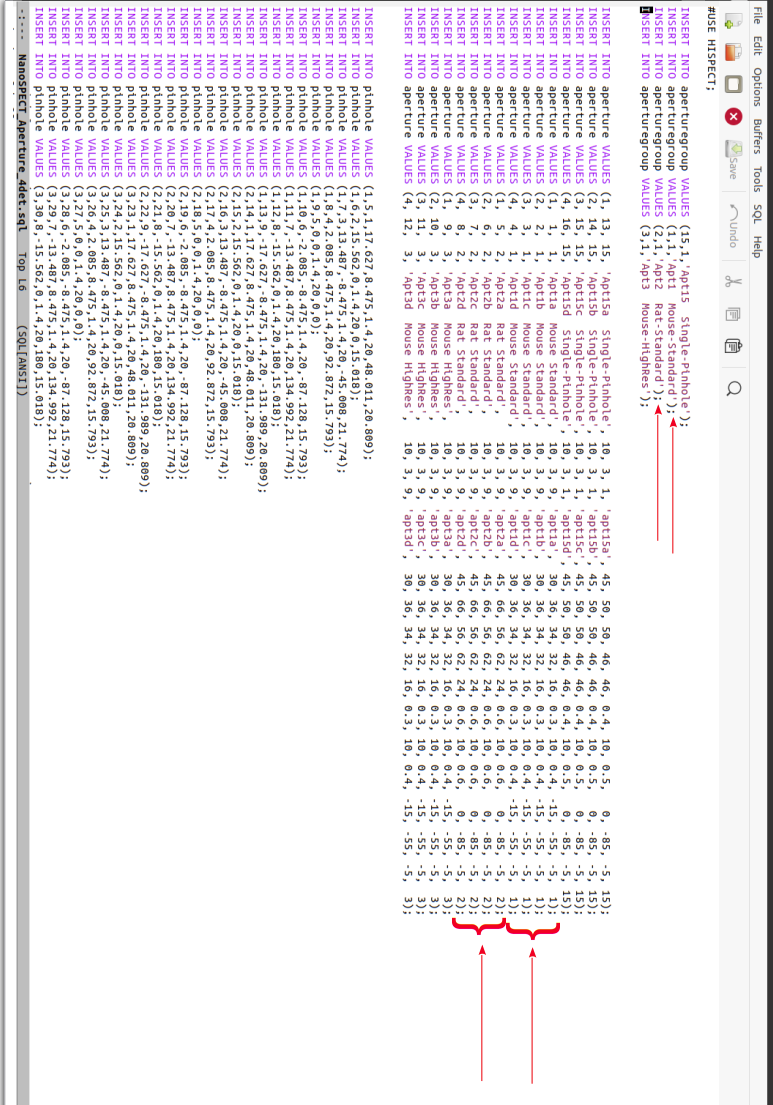
\includegraphics[scale=0.45]{figs/HiSPECT4det.png}
\caption{Part of \texttt{NanoSPECT\_Aperture\_4det.sql} file with important lines highlighted}
\label{fig:HiSPECT4det}
\end{figure}

\begin{figure}[htp]
\centering
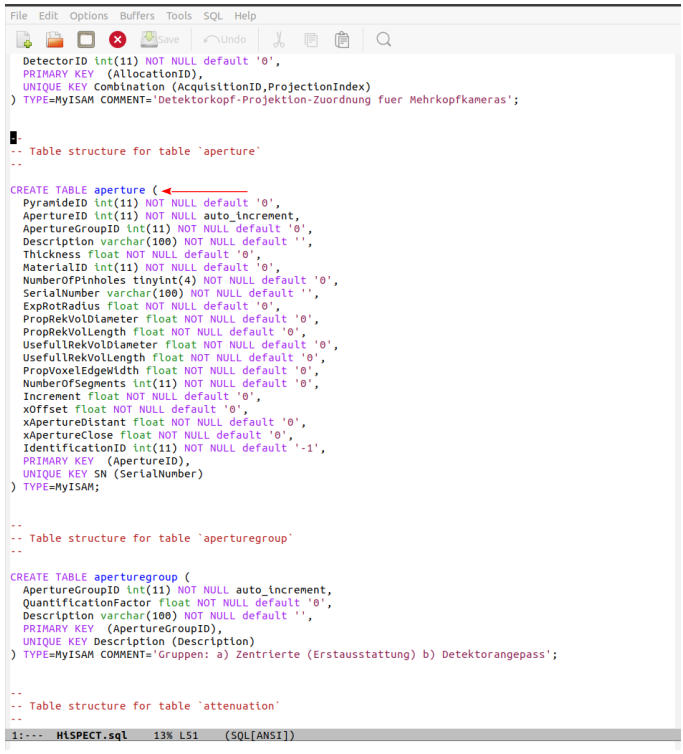
\includegraphics[scale=0.6]{figs/HiSPECTaperture.png}
\caption{Part of \texttt{HiSPECT.sql} file with important lines highlighted}
\label{fig:HiSPECTaperture}
\end{figure}


\begin{figure}[htp]
\centering
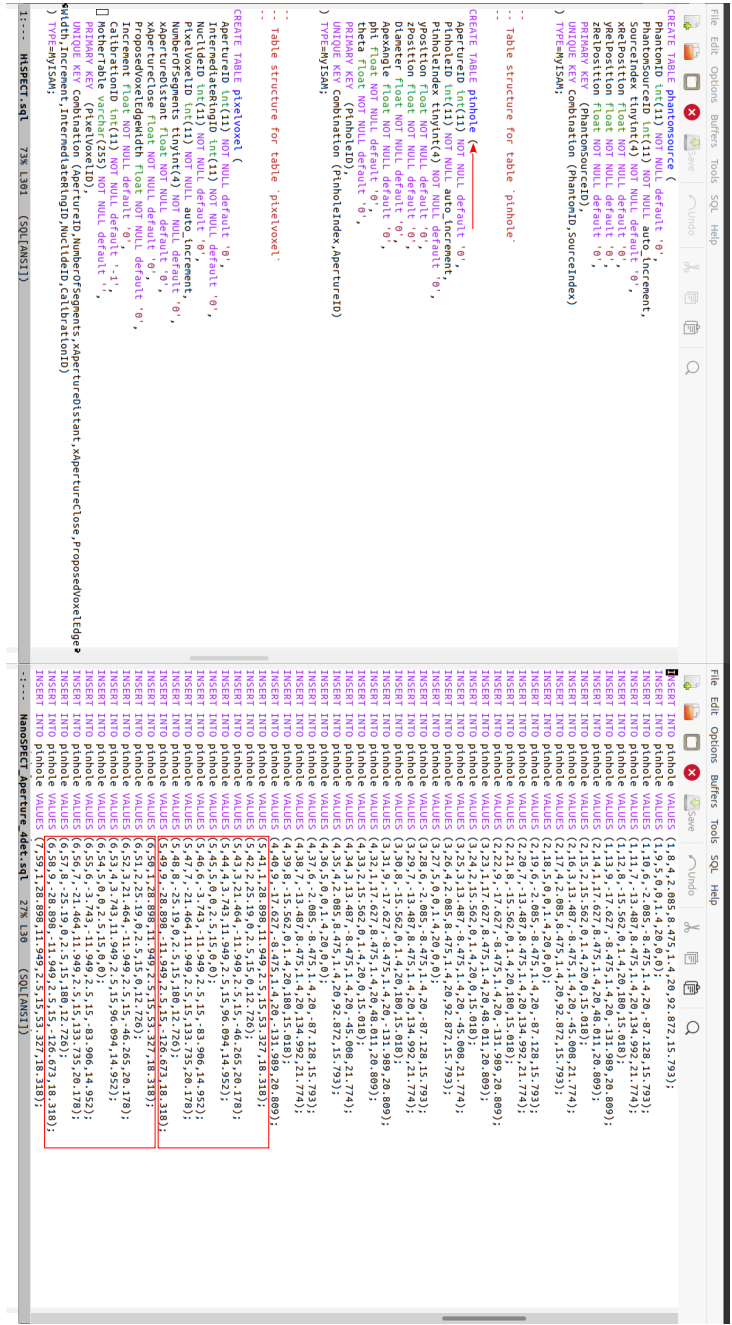
\includegraphics[scale=0.45]{figs/HiSPECTpinhole.png}
\caption{Part of \texttt{HiSPECT.sql} and \texttt{NanoSPECT\_Aperture\_4det.sql} file with important lines highlighted: parameters for APT1 are in blue rectangles and in red for APT2.}
\label{fig:HiSPECTpinhole}
\end{figure}

\clearpage
\subsection{HiSPECTtoGate tool}
This tool can be found on github: 

As input one should provide a text file obtained from HiSPECT (Figure~\ref{fig:HiSPECTpinhole}).


%\bibliographystyle{plain}
%\bibliography{biblio}



\end{document}